\documentclass[12pt]{report}
\usepackage{graphicx}
\usepackage{listings}
\lstset{numbers=left,firstnumber=auto}
\usepackage[margin=1in]{geometry}
\usepackage{amsmath, amsfonts, amsthm, titling, url, array}
\usepackage{mathtools}
\usepackage{hyperref}
\usepackage[table]{xcolor}
\usepackage{amssymb}
\usepackage{algorithm}
\usepackage[noend]{algpseudocode}

\usepackage{subfigure}

\makeatletter
\def\BState{\State\hskip-\ALG@thistlm}
\makeatother
\renewcommand{\algorithmicrequire}{\textbf{Input:}}
\renewcommand{\algorithmicensure}{\textbf{Output:}}
\newtheorem{theorem}{Theorem}
\theoremstyle{definition}
\newtheorem{definition}{Definition}


\usepackage{multirow}
\usepackage{booktabs}
\renewcommand*\familydefault{\sfdefault}

%\usepackage{amsart}
\usepackage{makecell}
\usepackage{boldline}

\usepackage{bm}%boldface math symbols


\usepackage{footnote}%savenote

%get rid of the red box of hyperlinks
\hypersetup{
	colorlinks,
	linkcolor={red!50!black},
	citecolor={blue!50!black},
	urlcolor={blue!80!black}
}

% Title Page
\title{PDE Project2 Report}
\author{Tu Yi\\Lei Qian}

\begin{document}
\maketitle

\section{Procudure}

We can know that $f(x,y)= sin(pi*x) * (pi^2 * y * (exp(y) - exp(1)) - (2*exp(y) + y* exp(y))) $.
Given the weights matrices for u and f, we can get the corresponding coefficient matrices A and C easily:\\
\begin{itemize}
	\item As for the coefficient matrix A of u takes the form:
	\begin{equation*}
	A = \frac{1}{6h^2} 
	\begin{pmatrix}
	B_1 & B_2 \\
	B_2 & B_1 & B_2 \\
	& \ddots & \ddots & \ddots \\
	&&B_2 & B_1 & B_2 \\
	&&&B_2 & B_1  \\
	\end{pmatrix}_{n^2 \times n^2}\\
	\end{equation*}
	
	where
	
	\begin{equation*}
	B_1 = \begin{pmatrix} 
	-20 & 4 \\
	4 & -20 & 4 \\
	& \ddots & \ddots & \ddots \\
	&&4 & -20 & 4 \\
	&&&4 & -20  \\
	\end{pmatrix}_{n \times n}\\
	B_2= \begin{pmatrix}
	4 & 1 \\
	1 & 4 & 1 \\
	& \ddots & \ddots & \ddots \\
	&&1 & 4 & 1 \\
	&&&1 & 4  \\
	\end{pmatrix}_{n \times n}\\
	\end{equation*}
	
	\item As for the coefficient matrix C of f takes the form:
	
	\begin{equation*}
	C = \frac{1}{12} 
	\begin{pmatrix}
	B_3 & I \\
	I & B_3 & I \\
	& \ddots & \ddots & \ddots \\
	&&I & B_3 & I \\
	&&&I & B_3  \\
	\end{pmatrix}_{n^2 \times n^2}\\
	\end{equation*}
	
	where
	
	\begin{equation*}
	B_3= \begin{pmatrix} 
	8 & 1 \\
	1 & 8 & 1 \\
	& \ddots & \ddots & \ddots \\
	&&1 & 8 & 1 \\
	&&8 & 1  \\
	\end{pmatrix}_{n \times n}\\
	\end{equation*}
\end{itemize}

So the equation becomes $Au = Cf$. Then we can use $u = A^{-1}Cf$ to calculate numerical solution.

\section{Result}
	\subsection{Grid Refinement Analysis}
	\begin{table}
		\caption{$Eh-h$}
		\begin{center}
			\begin{tabular}{c|c|c|c}
				%     \hline
				\textbf{n} & \textbf{h} & \textbf{Eh} & \textbf{Rate of Convergence}\\
				\hline
				&&&\\
				3 & $\frac{1}{4}$  & $1.5*10^{-3}$ &  \\
				&&&\\
				10 & $\frac{1}{11}$  & $2.527*10^{-6}$ & 4 \\
				&&&\\
				20 & $\frac{1}{21}$  & $1.920*10^{-6}$ & 4 \\
				&&&\\
				40 & $\frac{1}{41}$  & $1.324*10^{-7}$ & 4 \\
				
%				\hline
			\end{tabular}
		\end{center}
	\end{table}
	\subsection{Plot}


\begin{figure}[htbp]
	\centering
	\subfigure[v,n=20]{
		\begin{minipage}[t]{0.5\linewidth}
			\centering
			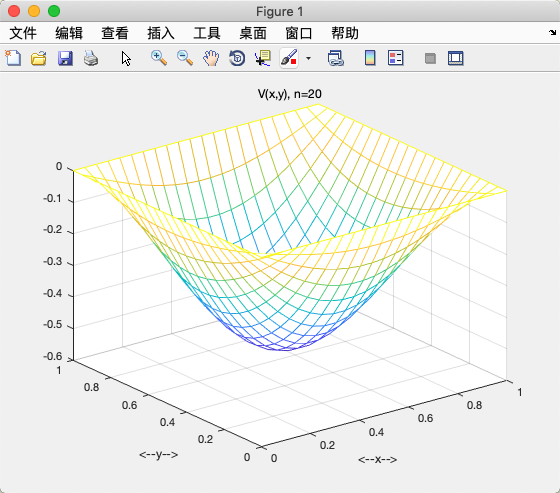
\includegraphics[width=\textwidth]{plot/vn20.png} 
			%\caption{fig1}
		\end{minipage}%
	}%
	\subfigure[u,n=20]{
		\begin{minipage}[t]{0.5\linewidth}
			\centering
			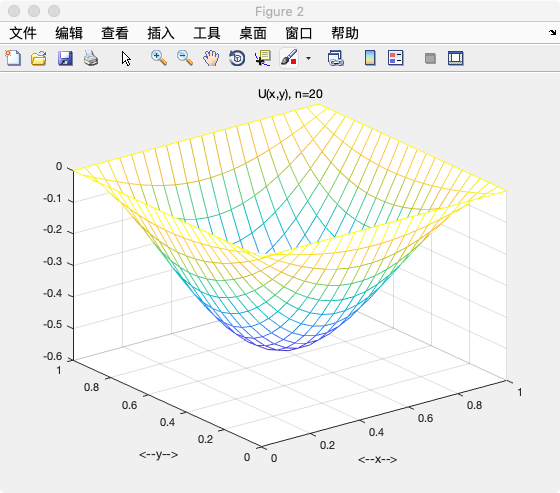
\includegraphics[width=\textwidth]{plot/un20.png} 
			%\caption{fig2}
		\end{minipage}%
	}%

	\centering
	\caption{n=20}
\end{figure}

\begin{figure}[htbp]
	\centering
	\subfigure[v,n=40]{
		\begin{minipage}[t]{0.5\linewidth}
			\centering
			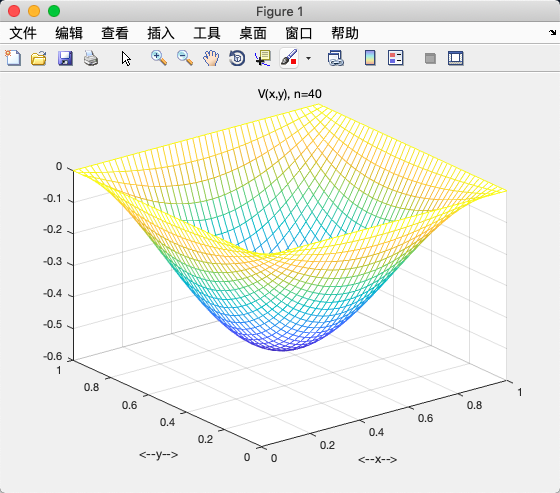
\includegraphics[width=\textwidth]{plot/vn40.png} 
			%\caption{fig1}
		\end{minipage}%
	}%
	\subfigure[u,n=40]{
		\begin{minipage}[t]{0.5\linewidth}
			\centering
			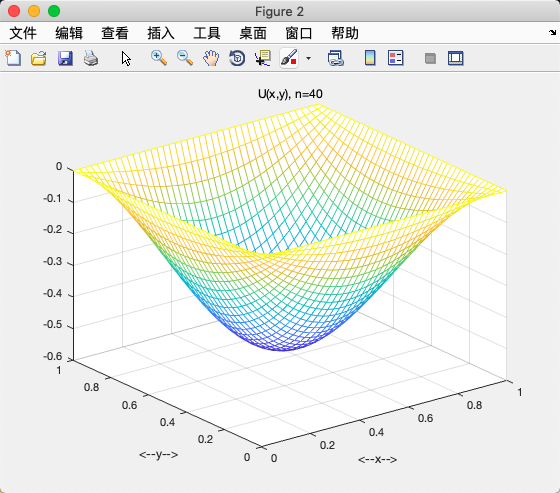
\includegraphics[width=\textwidth]{plot/un40.png} 
			%\caption{fig2}
		\end{minipage}%
	}%
	
	\centering
	\caption{ n=40}
\end{figure}
\vspace{2cm}
\section{Code}
	
	\lstinputlisting[language=MATLAB]{code/pde_proj2.m}
\end{document}         
